%==========================================================================
% Artigo (versão final) no template UNESC
% Baseado em: Exemplo de artigo cientifico UNESC (v1.0 - 25/06/2025)
%==========================================================================

%==========================================================================
% Pacotes utilizados pela UNESC - não delete as linhas abaixo
%==========================================================================
\documentclass{UNESC}
\usepackage[T1]{fontenc}
\usepackage[utf8]{inputenc}%\usepackage[latin1]{inputenc}
\renewcommand{\rmdefault}{phv} % Arial
\renewcommand{\sfdefault}{phv} % Arial
\usepackage[brazilian]{babel}
\usepackage{graphicx}
%\usepackage{subfigure}
\usepackage{hyperref}
\usepackage{quoting}
\usepackage[singlelinecheck=false]{caption}
\usepackage{enumitem}
\usepackage{float}

\hypersetup{
  setpagesize  = false,
  colorlinks   = true,    % Colours links instead of ugly boxes
  urlcolor     = blue,    % Colour for external hyperlinks
  linkcolor    = black,   % Colour of internal links
  citecolor    = black    % Colour of citations
}
\urlstyle{same}
\usepackage{setspace}

\usepackage[alf,recuo=0.0cm,abnt-emphasize=bf]{abntex2cite} 

%\captionsetup[figure]{justification=raggedright}


%==========================================================================
% Dados do artigo: título, autores e filiação
%==========================================================================
\title{DETECÇÃO DE REGRESSÕES VISUAIS EM INTEGRAÇÃO CONTÍNUA: IMPLEMENTAÇÃO E ANÁLISE DE TÉCNICAS PARA DETECTAR FALHAS DE INTERFACE}
\author
{
   Douglas Martignago Rosso\footnote{Curso de Ciência da Computação, Universidade do Extremo Sul Catarinense (Unesc), Criciúma - Santa Catarina - Brasil. douglasrosso10@gmail.com},
   Ana Cláudia Garcia Barbosa\footnote{Orientadora. Curso de Ciência da Computação, Universidade do Extremo Sul Catarinense (Unesc), Criciúma - Santa Catarina - Brasil. agb@unesc.net}
}
%==========================================================================
% Início do texto do artigo
%==========================================================================
\begin{document}

\onehalfspacing

\maketitle

\begin{abstract}
Este trabalho avalia técnicas de regressão visual em integração contínua, comparando diferença \emph{pixel a pixel}, métrica perceptual SSIM e abordagem por regiões com uso de máscaras. A verificação visual foi automatizada em \emph{pipelines} de CI/CD, com \emph{baseline} sob controle de versão e geração de relatório HTML e interface de revisão. Foram implementados doze cenários de mutação controlada e um cenário de controle, executados no \emph{viewport} de 1366\,×\,768\,px; a tela \emph{dashboard} foi capturada em três larguras de visualização. A comparação \emph{pixel a pixel} detectou oito dos doze cenários com mutação, a SSIM detectou cinco e a abordagem por regiões detectou nove. O estudo discute capacidade de detecção, ocorrência de alertas indevidos e esforço de triagem em variações de renderização, alterações de \emph{layout}, conteúdo dinâmico e responsividade. A combinação das três técnicas no mesmo fluxo apoia a decisão sobre aceitar ou rejeitar uma solicitação de mudança.
\end{abstract}

\vspace{1pt}

\begin{keywords}
regressão visual; integração contínua; testes automatizados; SSIM; baseline.
\end{keywords}

\vspace{1pt}

\begin{abstractinenglish}
{
This work evaluates visual regression techniques in continuous integration by comparing pixel-by-pixel diff, the SSIM perceptual metric, and a region-based approach with masking. Visual checks were automated in CI/CD pipelines, with baselines under version control and traceable artifacts (HTML report and a review UI). Twelve controlled mutation scenarios and one control scenario were implemented and executed across three viewport widths. The pixel-by-pixel comparison detected eight of twelve mutation scenarios, SSIM detected five, and the region-based approach detected nine, showing complementary sensitivity profiles. The study discusses detection capability, noisy alerts, and triage effort under rendering variability, layout changes, dynamic content, and responsiveness. Combining the three techniques in the same workflow supports accept/reject decisions in pull requests.
}
\end{abstractinenglish}

\vspace{1pt}

\begin{keywordsenglish}
{visual regression; continuous integration; automated testing; SSIM; baseline.}
\end{keywordsenglish}


\section{INTRODUÇÃO}

A qualidade visual de interfaces web é uma preocupação em equipes que adotam ciclos curtos de entrega. Mudanças de código como ajustes de espaçamento, troca de fontes ou alteração de cores podem modificar a aparência da interface sem afetar a lógica funcional. Quando a versão atual diverge da referência aprovada, ocorre uma regressão visual: uma diferença indesejada identificada pela comparação de imagens de tela. A verificação manual de cada tela em cada dispositivo consome tempo e está sujeita a falhas humanas, o que motiva o uso de técnicas automatizadas em fluxos de Integração e Entrega Contínuas (CI/CD) \cite{shahin2017}. No recorte de regressão visual, o objetivo é indicar se as mudanças de código afetam padrões de apresentação por meio da comparação de imagens entre versões \cite{tanno2020,figueiredo2018,bordignon2019}.

As abordagens para essa verificação se organizam em três grupos. A comparação \emph{pixel a pixel} identifica qualquer diferença entre as imagens, mas tende a gerar mais alertas quando há variações de renderização, de fonte ou de \emph{layout} \cite{figueiredo2018,tanno2020}. As métricas perceptuais, como a SSIM (\emph{Structural Similarity Index}) proposta por \citeonline{wang2004}, comparam luminância, contraste e estrutura, com resultado próximo da percepção humana. A MS-SSIM amplia essa ideia para múltiplas escalas \cite{wang2003msssim}. A abordagem por regiões divide a tela em partes, compara áreas equivalentes e permite mascarar conteúdo dinâmico, o que reduz o efeito de deslocamentos e auxilia a triagem \cite{tanno2020}.

Elementos variáveis (datas, contadores, dados externos) produzem diferenças recorrentes se não tratados. Recomenda-se aplicar máscaras apenas em regiões inevitavelmente variáveis e adotar política explícita de atualização de \emph{baseline}, para preservar rastreabilidade e não normalizar defeitos \cite{tanno2020,heinonen2020}. \citeonline{heinonen2020} aponta que o determinismo operacional exige versões fixas de sistema e navegador, resolução e densidade constantes, fontes empacotadas, idioma e fuso horário controlados, animações desativadas e simulação de dados quando necessário. A integração da verificação visual ao fluxo de CI/CD vincula imagens de referência, diferenças e relatórios a \emph{commits} e solicitações de mudança, em linha com práticas de entrega incremental documentadas por \citeonline{shahin2017}. No âmbito nacional, \citeonline{santos2022} constatou que equipes brasileiras ainda recorrem predominantemente a testes manuais, enquanto \citeonline{pinheiro2015} mostrou que a automação de testes de aceitação em aplicações web reduz o esforço de verificação e o retrabalho com defeitos descobertos tardiamente. No contexto específico da integração contínua, \citeonline{lima2023} mostrou que técnicas adaptativas de priorização de casos de teste permitem reduzir o tempo de \emph{feedback} nos ciclos de CI ao selecionar os testes mais informativos para cada \emph{build}.

\citeonline{tanno2020} comparam técnicas de detecção de regressão visual em aplicações web, avaliando comparação \emph{pixel a pixel}, abordagens por regiões com segmentação da tela e métricas perceptuais. O estudo identifica que a comparação direta de pixels é sensível a flutuações de renderização e que abordagens por regiões reduzem o impacto de deslocamentos ao segmentar a tela em partes independentes. Os autores recomendam mascaramento de áreas dinâmicas e política explícita de atualização de \emph{baseline} para evitar acúmulo de alertas. Contudo, o trabalho não executa cenários de mutação controlada com coleta padronizada de métricas por técnica, nem integra as verificações a um \emph{pipeline} de CI/CD com artefatos rastreáveis. Essa lacuna é diretamente abordada pelo presente trabalho, que confronta as três técnicas sob mesma calibração em treze cenários rotulados e vincula os resultados a um fluxo de CI/CD rastreável.

\citeonline{heinonen2020} investiga a integração de testes visuais em \emph{pipelines} de integração contínua, discutindo práticas de determinismo operacional, versões fixas de navegador, resolução constante, desativação de animações para reduzir variações entre capturas. O estudo estabelece que o determinismo do ambiente é pré-requisito para a confiabilidade dos resultados, mas não compara o desempenho das técnicas de comparação entre si, nem avalia cenários específicos de mutação com coleta de métricas por técnica. O presente trabalho aplica as recomendações de determinismo operacional de \citeonline{heinonen2020} e as estende com a comparação experimental entre pixel, SSIM e regiões em cenários controlados.

No contexto nacional, \citeonline{figueiredo2018} avalia a aplicação de testes regressivos visuais em um projeto Android com Appium, demonstrando a viabilidade da abordagem em ambientes móveis, mas sem integração a um \emph{pipeline} de CI/CD e sem comparação entre técnicas distintas de comparação de imagem. \citeonline{bordignon2019} analisa ferramentas visuais de teste de interfaces gráficas voltadas à verificação de requisitos não funcionais, identificando diferenças entre as ferramentas disponíveis sem conduzir cenários de mutação controlada com coleta quantitativa de métricas por técnica. Ambos os trabalhos demonstram a relevância da verificação visual de interfaces no cenário brasileiro, mas não comparam as abordagens de pixel, SSIM e regiões sob mesma calibração, nem integram os resultados a um fluxo rastreável de CI/CD.

Na literatura consultada para este trabalho, não foram identificados estudos que comparem, sob condições controladas, as três principais técnicas (pixel a pixel, SSIM e regiões) quanto à capacidade de detecção, à incidência de alertas indevidos e ao suporte à triagem, com artefatos rastreáveis em CI/CD, combinando cenários de mutação controlada, coleta padronizada de métricas por técnica e evidências vinculadas ao histórico de versões em diferentes larguras de visualização.

Este trabalho avalia três técnicas de regressão visual em um fluxo automatizado de CI/CD. Para isso, foi implementada a ferramenta PixelGuard, distribuída como pacote npm, que integra captura de telas via Playwright, comparação pelas três técnicas em paralelo e publicação de evidências (relatório HTML e interface de revisão). Foram construídos doze cenários de mutação controlada e um cenário de controle, executados no \emph{viewport} fixo de 1366\,×\,768\,px, com a tela \emph{dashboard} avaliada adicionalmente em três larguras de visualização, com imagens de referência sob controle de versão.

A hipótese do trabalho é que a combinação das três técnicas em um único fluxo rastreável de CI/CD proporciona cobertura complementar de tipos de regressão visual, reduzindo o risco de falsos negativos em relação ao uso isolado de qualquer uma delas.

O objetivo geral deste trabalho é avaliar técnicas de regressão visual quanto à detecção de falhas, à ocorrência de falsos positivos e ao esforço de triagem, com imagens de referência sob controle de versão em CI/CD. Como objetivos específicos, pretende-se identificar cenários e tipos de mudança na interface com risco de regressão visual, implementar um fluxo automatizado de verificação em CI/CD com geração de artefatos rastreáveis, medir o desempenho das técnicas em detecção, falsos positivos e esforço de triagem, e analisar a robustez diante de variações de renderização, \emph{layout} e conteúdo dinâmico.


\section{MATERIAIS E MÉTODOS}

Esta pesquisa é de natureza aplicada, pois compara técnicas de detecção de regressão visual e as integra a fluxos de Integração e Entrega Contínuas (CI/CD). Quanto aos objetivos, adota procedimentos experimentais e descritivos: experimental por aplicar mutações controladas e coletar métricas quantitativas por técnica em cenários rotulados; e descritiva por relatar os indicadores produzidos. Tem caráter exploratório nos parâmetros de ajuste dos limiares, para os quais não há valores prescritos na literatura, razão pela qual os valores adotados são registrados como pontos de partida configuráveis. Como base conceitual, adotam-se métricas perceptuais de imagem, em especial a SSIM, proposta por \citeonline{wang2004}, e práticas de operação em \emph{pipelines} de software discutidas por \citeonline{shahin2017} e \citeonline{heinonen2020}.

\subsection{AMBIENTE EXPERIMENTAL E DETERMINISMO}
Os testes foram executados em ambiente padronizado para garantir resultados reprodutíveis. Utilizou-se Node.js (v24) e Playwright (Chromium em modo \emph{headless}) para captura de telas, com densidade de pixels fixa, idioma pt-BR e fuso horário America/Sao\_Paulo. Para reduzir instabilidades, o relógio do sistema e a função \texttt{Math.random} foram congelados por um \emph{script} de inicialização injetado antes do carregamento da página, mantendo constantes os valores dinâmicos (data, hora, números aleatórios) entre execuções. Após o carregamento completo da página, animações e transições CSS foram desativadas por injeção de folha de estilo, garantindo que a captura registrasse a interface em estado estático. Na comparação principal com a tela \emph{dashboard}, as capturas foram feitas em página inteira; nos cenários de mutação, utilizou-se captura pela área do \emph{viewport}, sem \emph{full-page}, para eliminar variações de dimensão entre execuções. As imagens atuais foram salvas em diretório dedicado. As imagens de referência (\emph{baseline}) ficaram em diretório próprio sob controle de versão, permitindo auditoria e rastreabilidade.

\subsection{DELINEAMENTO EXPERIMENTAL}
O experimento combina quatro elementos:
\begin{enumerate}[label=\alph*),leftmargin=1.5em]
  \item Cenário avaliado. O cenário central foi uma aplicação de página única (\emph{single-page}) em React (tela \textit{dashboard}), capturada de forma determinística para reduzir variações entre execuções. Mesmo assim, registrou-se um caso de instabilidade: pequenas diferenças de altura entre capturas de página inteira na mesma largura, que afetam a comparabilidade.
  \item Técnicas. Foram comparadas três abordagens. A primeira é a comparação \emph{pixel a pixel} com tolerância, usando a biblioteca pixelmatch. A segunda é a comparação perceptual baseada em SSIM, conforme \citeonline{wang2004}, com implementação própria em blocos não sobrepostos. A terceira é a abordagem por regiões com segmentação em grade e suporte a máscaras por célula para áreas dinâmicas \cite{tanno2020}. Nesta implementação, o suporte a mascaramento espacial está disponível apenas na técnica por regiões; as comparações pixel e SSIM avaliam a imagem inteira sem exclusão de regiões.
  \item Larguras de visualização. Foram utilizados três \emph{viewports}: 360\,px (\textit{mobile}), 768\,px (\textit{tablet}) e 1366\,px (\textit{desktop}). Cada página foi capturada em todas as larguras.
  \item Máscaras e política de aceitação. A técnica por regiões foi configurada com grade 4\,$\times$\,6 e suporte a mascaramento por célula. Para a tela \textit{dashboard}, as máscaras permaneceram desativadas (lista vazia) para evidenciar o comportamento de ruído e alertas em condição padrão. No conjunto de cenários, o cenário de conteúdo dinâmico foi executado em duas variantes (sem máscara e com máscara aplicada à célula que contém o valor variável), justamente para isolar o efeito do mascaramento. A atualização de \emph{baseline} foi tratada como processo explícito e rastreável no fluxo de CI/CD.
\end{enumerate}

\subsection{IMPLEMENTAÇÃO DO FLUXO (PIXELGUARD)}
Para a avaliação e a operação em \emph{pipeline}, foi implementada a ferramenta PixelGuard, distribuída como pacote npm. A ferramenta cobre três etapas principais. A primeira é a captura de telas com Playwright em ambiente controlado, com relógio e Math.random congelados, animações desativadas e idioma e fuso horário fixos. A segunda é a comparação em paralelo pelas três técnicas, com limiares definidos em arquivo de configuração. A comparação \emph{pixel a pixel} usa tolerância de 0,1 e limite de 0,1\% de diferença, a SSIM usa limiar mínimo 0,99 e bloco 8, e a comparação por regiões usa grade 4\,$\times$\,6 e limite de 1,0\% por célula. A terceira etapa é a geração de evidências em relatório HTML autocontido e em interface de revisão em React, que permite inspecionar cada comparação lado a lado, em sobreposição ou com controle deslizante.

No fluxo de CI/CD, foram criados três fluxos de trabalho no GitHub Actions. O primeiro executa a verificação visual em cada solicitação de mudança. O segundo controla o resultado por comentário, com as ações aprovar, rejeitar ou redefinir. O terceiro atualiza as imagens de referência após a integração no ramo principal. A interface de revisão se comunica com a API de \emph{Statuses} do GitHub para definir o estado do \emph{commit} como sucesso, falha ou pendente. Detalhes de instalação, comandos da interface de linha de comando, opções de configuração e exemplos de uso estão documentados no README do pacote, no repositório.


\subsection{AVALIAÇÃO POR CENÁRIOS DE REGRESSÃO}
Além da comparação com a tela \textit{dashboard}, foram implementadas doze páginas de cenário na aplicação, cada uma projetada para isolar um tipo de alteração e expor pontos fortes e fracos de cada técnica. A cada cenário corresponde uma mutação controlada, injetada via CSS ou \emph{script} durante a captura, e uma imagem de referência capturada nas mesmas condições, exceto pela mutação. Os cenários utilizaram \emph{viewport} fixo de 1366\,$\times$\,768\,px (captura por área do \emph{viewport}, sem \emph{full-page}) para eliminar variações de dimensão entre capturas. Um cenário adicional de controle (imagem idêntica) foi incluído para verificar a ausência de falsos positivos.

A escolha dos cenários baseou-se nos tipos de defeito visual recorrentes na literatura \cite{tanno2020,figueiredo2018,heinonen2020} e nos eixos em que as três técnicas apresentam comportamento distinto: amplitude da alteração, extensão espacial, natureza (cor, posição, texto, transparência, sombra) e origem (mutação controlada ou variação natural). Cenários cromáticos que preservam estrutura (cor sutil, borda fina) separam o comportamento da SSIM do comportamento de pixel e regiões; alterações estruturais espalhadas (deslocamento, tipografia, troca de fonte) testam a reatividade conjunta das três técnicas; cenários de baixa amplitude (opacidade, sombra) expõem o limite inferior de detecção; o cenário de conteúdo dinâmico avalia o suporte a mascaramento; e o controle verifica a ausência de falso positivo.

Os cenários são:
\begin{enumerate}[label=\alph*),leftmargin=1.5em]
  \item Mudança sutil de cor: alteração do tom de dois cards em uma grade de seis, com diferença de 22 a 37 unidades RGB por canal. Avalia sensibilidade a variações cromáticas que preservam a composição estrutural.
  \item Deslocamento de \emph{layout}: inserção de 24\,px de margem superior na primeira seção de conteúdo, deslocando as demais para baixo.
  \item Variação tipográfica: aumento de letter-spacing em blocos de texto, produzindo diferenças de anti-aliasing distribuídas sem alterar a estrutura de \emph{layout}.
  \item Conteúdo dinâmico: captura de referência com congelamento de Date e Math.random versus captura atual sem congelamento, de modo que valores dinâmicos (data, hora, contadores) diferem naturalmente. Executado sem máscaras e com máscaras nas células que contêm conteúdo variável.
  \item Alteração localizada de componente: modificação do texto e da cor de borda de um único card em grade de seis, mantendo os demais inalterados.
  \item Opacidade e transparência: redução de opacity para 0,92 em três de seis cards com fundo colorido, produzindo mudança uniforme e sutil em muitos pixels simultaneamente.
  \item Sombra e elevação: adição de box-shadow em três de seis cards planos, criando gradientes suaves nas bordas sem alterar conteúdo nem posicionamento.
  \item Micro-deslocamento (1\,px): inserção de apenas 1\,px de margem superior na primeira seção, testando o limiar mínimo de detecção de cada técnica.
  \item Alteração de borda fina: troca de cor de border (2\,px) em dois de seis cards, afetando poucos pixels mas modificando a identidade visual do componente.
  \item Remoção de elemento: ocultação (display: none) de um card em grade de seis, provocando reposicionamento de elementos adjacentes e espaço vazio.
  \item Troca de família de fonte: substituição da font-family de dois blocos de texto por fonte serifada, alterando métricas tipográficas (largura de glifos, \emph{kerning}) sem mudar o tamanho nominal.
  \item Imagem idêntica (controle): captura de página estática sem mutação em baseline e current, ambas com congelamento. Avalia se alguma técnica produz falso positivo.
\end{enumerate}

Para cada cenário, as imagens foram comparadas pelos três métodos com os mesmos limiares da avaliação principal.

\subsection{MÉTRICAS E COLETA}
Foram coletados indicadores gerados automaticamente pelas técnicas e pelo próprio fluxo de execução. Para a comparação \emph{pixel a pixel}, registrou-se o percentual de pixels diferentes e a contagem de pixels divergentes. Para a SSIM, registrou-se a pontuação de similaridade estrutural e a proporção de blocos com baixa similaridade. Para a abordagem por regiões, registraram-se a quantidade de células reprovadas e o total de células, além do percentual de diferença por célula. Também foram registrados erros operacionais (por exemplo, dimensões diferentes entre \emph{baseline} e captura atual) e o tempo de execução por técnica. A análise comparou esses indicadores entre técnicas e entre as larguras de visualização (\textit{mobile}, \textit{tablet} e \textit{desktop}), considerando tanto a sensibilidade quanto a leitura das evidências geradas.

\subsection{VALIDADE E LIMITAÇÕES}
Foram documentadas ameaças à validade interna, como viés na seleção de telas e sensibilidade dos limiares de aceitação, e à validade externa, como o alcance da generalização para outros tipos de aplicações e ambientes. Também foram registradas dependências do ambiente (fontes, motores de renderização e resolução) e as medidas adotadas para evitar que variações não controladas afetassem os resultados. No uso de máscaras, optou-se por restringi-las a regiões inevitavelmente variáveis e revisá-las a cada atualização de \emph{baseline}, evitando que um ajuste inadequado escondesse defeitos. Outras três limitações do recorte adotado merecem registro. A primeira é que a avaliação multi-\emph{viewport} se restringe à tela \textit{dashboard}, enquanto os doze cenários de mutação controlada foram executados apenas no \emph{viewport} de 1366\,$\times$\,768\,px, para eliminar variações de dimensão entre capturas. A segunda é que o esforço de triagem foi avaliado de forma qualitativa, a partir das evidências geradas pelo fluxo, sem cronometragem com avaliadores. A terceira é que os indicadores de taxa de detecção e taxa de alertas indevidos são reportados em relação ao conjunto rotulado de cenários construídos para este estudo, e não em relação a um histórico de alterações reais de produção.


\section{RESULTADOS E DISCUSSÃO}

A execução automatizada do fluxo produziu dois conjuntos de resultados. A tela \textit{dashboard} foi capturada nas três larguras de visualização (\textit{mobile} a 360\,px, \textit{tablet} a 768\,px e \textit{desktop} a 1366\,px) e comparada com a respectiva imagem de referência, verificando a estabilidade do fluxo em operação normal. Em seguida, foram executados os doze cenários de mutação controlada e o cenário de controle no \emph{viewport} de 1366\,$\times$\,768\,px para medir a capacidade de detecção de cada técnica.

A comparação \emph{pixel a pixel} reprovou oito dos doze cenários com mutação, a SSIM reprovou cinco e a abordagem por regiões reprovou nove. O cenário de controle foi aprovado pelas três técnicas, sem registro de falso positivo. Os indicadores foram extraídos automaticamente pelo PixelGuard e gravados em \emph{results/results.json} (avaliação principal) e \emph{results/scenarios/scenarios-results.json} (avaliação por cenários), com veredito (PASS ou FAIL), métrica principal de cada técnica e tempo de execução. Os limiares utilizados na decisão automática foram os definidos na configuração: 0,1\,\% para pixel, 0,99 para SSIM e 1,0\,\% por célula na abordagem por regiões.

\subsection{JUSTIFICATIVA DOS LIMIARES ADOTADOS}
Os parâmetros de aceitação de cada técnica foram definidos como pontos de partida configuráveis, combinando padrões das bibliotecas utilizadas e escolhas de projeto. Não foi conduzida varredura sistemática dos limiares (por exemplo, curva ROC sobre conjunto rotulado), limitação registrada na seção de validade.

Para a comparação \emph{pixel a pixel}, adotou-se tolerância de 0,1 por canal, valor padrão da biblioteca pixelmatch e limite global de 0,1\,\% de pixels diferentes. Em uma captura de 1366\,$\times$\,768\,px, esse percentual corresponde a aproximadamente 1.049 pixels divergentes; o valor é um ponto de partida, não um ótimo proposto.

Para a SSIM, adotou-se limiar mínimo de 0,99 e janela de bloco de 8\,$\times$\,8\,px. O limiar não é prescrito por \citeonline{wang2004} e foi escolhido por situar-se imediatamente abaixo de 1, compatível com a expectativa de quase-igualdade entre \emph{baseline} e captura atual. O cenário de alteração de componente obteve SSIM 0,9924, valor acima do limiar de 0,99, e recebeu veredito PASS conforme esperado; o resultado é coerente com a caracterização de \citeonline{wang2004}, pois a alteração é cromática e não afeta a estrutura perceptual da cena.

Para a abordagem por regiões, adotou-se grade de 4\,$\times$\,6 (24 células) e limite de 1,0\,\% por célula dez vezes mais permissivo do que o limite global de pixel, pois variações localizadas ocupam proporção maior dentro de uma célula do que sobre a imagem inteira. Todos os parâmetros são expostos em \emph{pixelguard.config.js} e podem ser substituídos por calibração específica à aplicação.

\subsection{RESUMO NUMÉRICO DAS COMPARAÇÕES}
A Tabela \ref{tab:resumo-resultados} compara a \emph{baseline} aprovada com a captura recém-gerada da tela \textit{dashboard} nas três larguras de visualização. A coluna \emph{Pixel} indica o percentual de pixels divergentes (PASS ≤ 0,1\,\%); a coluna \emph{SSIM} indica a pontuação de similaridade estrutural entre 0 e 1 (PASS ≥ 0,99); e a coluna \emph{Regiões} indica a fração de células reprovadas em grade 4\,$\times$\,6 (PASS = 0 células acima de 1\,\% de diferença interna).

\vspace{0.2cm}
\begin{table}[H]
\centering
\captionlistentry{}
Tabela \thetable  \hspace{0.5pt} - {Resumo das comparações da tela \textit{dashboard}}
\label{tab:resumo-resultados}
\resizebox{\textwidth}{!}{%
\begin{tabular}{p{6cm}|c|c|c}
\hline
\multicolumn{4}{c}{\textbf{Resumo das comparações da tela dashboard}} \\
\hline
\textbf{Imagem} & \textbf{Pixel} & \textbf{SSIM} & \textbf{Regiões} \\
\hline
dashboard-desktop-1366w & PASS (0\%) & PASS (1,0000) & PASS (0/24) \\
\hline
dashboard-mobile-360w & PASS (0\%) & PASS (1,0000) & PASS (0/24) \\
\hline
dashboard-tablet-768w & PASS (0\%) & PASS (1,0000) & PASS (0/24) \\
\hline
\end{tabular}%
}
\vspace{-0.3cm}
\flushleft
\hspace{0cm}\footnotesize Fonte: Do autor.
\end{table}

Nos três \emph{viewports} não foram observados pixels diferentes, a pontuação SSIM permaneceu em 1,0 e nenhuma região foi reprovada (0/24). Quando a captura é gerada nas mesmas condições da \emph{baseline}, o fluxo não acusa diferença, mesmo executando três comparações independentes. \citeonline{heinonen2020} estabelece como pré-requisito de operação em \emph{pipelines} que o ambiente de captura seja determinístico; sem esse controle, a comparação \emph{pixel a pixel} acumula falsos positivos e perde utilidade prática. No experimento, o congelamento de \emph{Date} e de \emph{Math.random} antes do carregamento da página, somado à execução em modo \emph{headless} com densidade de pixels fixa, garantiu que duas execuções consecutivas produzissem imagens binariamente equivalentes.

Quanto ao custo operacional, com base nos campos \emph{executionMs} de \emph{scenarios-results.json}, o tempo médio por comparação ficou em 134\,ms para a técnica \emph{pixel a pixel}, 134\,ms para a SSIM e 122\,ms para a abordagem por regiões. Como as três técnicas são executadas em paralelo, o tempo total de comparação por captura fica abaixo de 200\,ms, o que torna o fluxo viável para execução em cada solicitação de mudança sem impacto mensurável no tempo total do \emph{pipeline} de CI/CD.

\subsection{EVIDÊNCIAS VISUAIS E TRIAGEM}
O fluxo gerou imagens de diferenças para as três técnicas (pixel, SSIM e regiões), além de um relatório HTML com resumo e evidências. A interface de revisão (\emph{Review UI}) foi utilizada para suportar a triagem, permitindo selecionar uma captura e alternar entre técnicas de \emph{diff}. A Figura~\ref{fig:diff-comparativo} reúne, lado a lado, o painel de comparação do cenário \emph{Mudança sutil de cor} nas três técnicas (pixel, SSIM e regiões), facilitando a leitura conjunta das evidências.

\begin{figure}[H]
\begin{center}
\captionlistentry{}
Figura \thefigure \hspace{1pt} - Painéis de comparação lado a lado: pixel, SSIM e regiões (cenário \emph{Mudança sutil de cor})
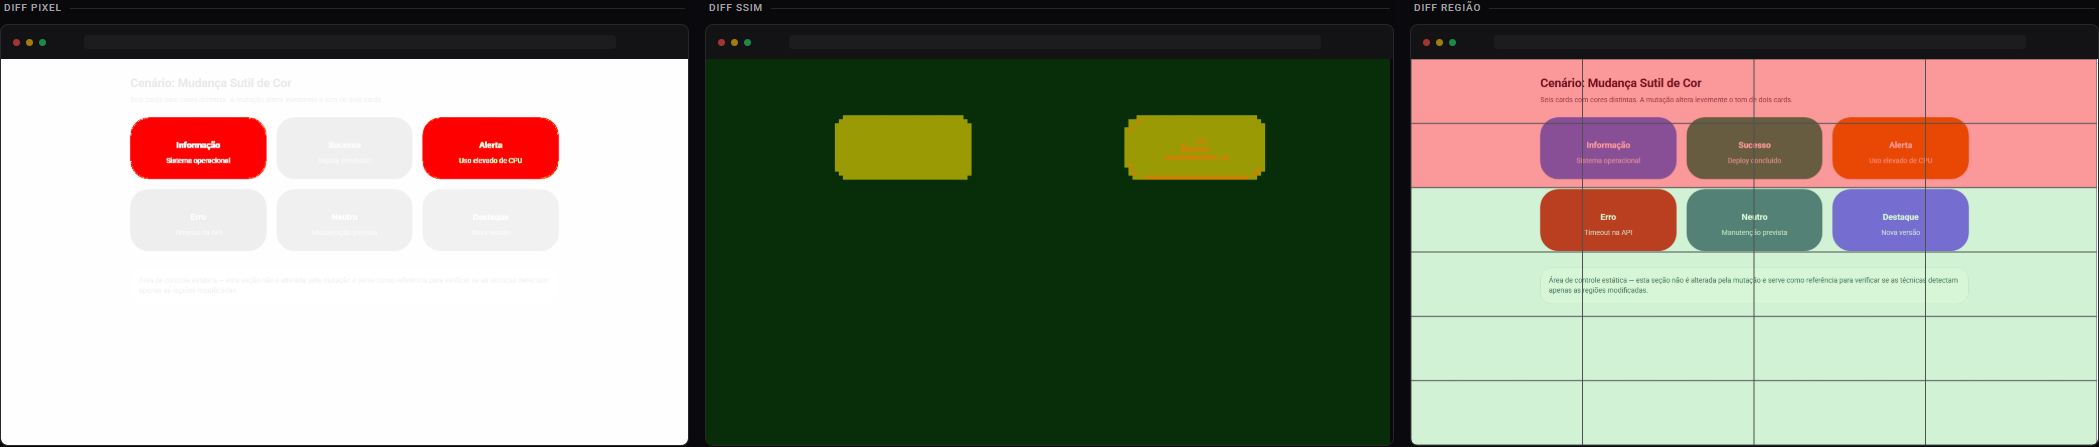
\includegraphics[width=\linewidth]{Figs/03-diff-comparativo.png}
\label{fig:diff-comparativo}
\end{center}
\flushleft
\vspace{-0.5cm}
\hspace{0.08cm} \footnotesize{ Fonte: Do autor.}
\end{figure}

No painel da esquerda (pixel), as duas regiões em vermelho correspondem aos cards cujo tom foi alterado, e o restante da imagem permanece preto, indicando que apenas esses pixels diferiram da \emph{baseline}. O número associado (5,854\,\% de pixels diferentes) é alto em comparação ao limiar de 0,1\,\%, e por isso a técnica reprovou. No painel central (SSIM), as áreas claras representam blocos onde a similaridade estrutural caiu. Como a alteração foi de cor e não de estrutura (forma, contorno, texto), a queda foi pequena, com pontuação 0,9976 acima do limiar de 0,99, e a técnica aprovou a mudança, embora ela seja visível a olho nu. No painel da direita (regiões), as oito células em vermelho indicam quais quadrantes da grade 4\,$\times$\,6 ultrapassaram o limite de 1\,\% de diferença interna. As outras dezesseis permanecem azuladas, sinalizando \emph{passed}.

A SSIM isolada não acusaria a regressão, o pixel isolado mostraria o problema sem indicar em que região da imagem ocorre, e a abordagem por regiões localizaria sem informar a magnitude perceptual. \citeonline{tanno2020} discutem essa limitação ao apontar que a comparação direta de pixels é sensível a flutuações de renderização e que a abordagem por regiões agrega contexto espacial à decisão. A figura ilustra, em um único caso, a vantagem de combinar os três indicadores em vez de escolher um deles isoladamente.

\subsection{DISCUSSÃO: SENSIBILIDADE, RUÍDO E OPERAÇÃO EM CI/CD}
Os dados de \emph{scenarios-results.json} expõem três comportamentos para a operação da verificação visual: a sensibilidade de cada técnica a diferentes tipos de mudança, a ocorrência de ruído (alertas sem regressão real correspondente) e o impacto desse conjunto na rotina de CI/CD.

Em termos de sensibilidade, a comparação \emph{pixel a pixel} foi a mais reativa a alterações pequenas. Quando a interface foi modificada apenas no texto e na borda de um único componente, a técnica registrou 0,128\,\% de pixels diferentes, percentual baixo em termos absolutos, mas suficiente para acionar o alerta por ultrapassar o limiar de 0,1\,\%. O mesmo ocorreu no micro-deslocamento de 1\,px, em que apenas uma linha de pixels foi deslocada e a técnica acusou 0,198\,\% de diferença. O comportamento concorda com \citeonline{figueiredo2018} e \citeonline{tanno2020}, que apontam a comparação direta de pixel como sensível a qualquer alteração, vantagem para não perder regressões reais e origem dos alertas espúrios quando há flutuação de renderização ou anti-aliasing entre execuções.

A SSIM teve comportamento distinto porque não conta pixels, mas avalia se a estrutura (forma, contornos, contraste) das duas imagens permanece equivalente em pequenas janelas. Além da pontuação global, a técnica registra a quantidade de blocos de 8\,$\times$\,8\,px com baixa similaridade, em relação ao total de 16.320 blocos por captura. Nos cenários em que a estrutura foi afetada, a pontuação caiu de forma marcada e a proporção de blocos com baixa similaridade subiu, com 0,8762 e 25,23\,\% no deslocamento de \emph{layout} (toda a parte inferior da página foi empurrada 24\,px para baixo, deformando a relação entre os elementos), 0,9269 e 9,33\,\% na variação tipográfica (o aumento de \emph{letter-spacing} alterou o desenho de cada linha de texto), 0,9316 e 15,30\,\% no micro-deslocamento (a translação afeta a relação espacial dos blocos) e 0,8886 e 15,21\,\% na troca de fonte (mudou o desenho dos glifos). Nos cenários em que apenas a aparência local mudou sem alterar estrutura, como a redução de opacidade e a adição de sombra, a SSIM permaneceu acima de 0,995 e a proporção de blocos com baixa similaridade ficou em 0\,\% e 2,85\,\%, respectivamente, dentro do limite de tolerância. O comportamento confirma a proposta de \citeonline{wang2004}, em que a SSIM, por ser perceptual, ignora variações de baixa intensidade visual que não modificam a leitura estrutural da cena, ainda que a diferença seja perceptível.

A abordagem por regiões cumpriu um papel diferente das outras duas. Além do veredito, ela indica em quais células da grade 4\,$\times$\,6 a diferença ocorreu, e qual o percentual de divergência em cada uma delas. Em cenários como remoção de elemento e alteração de componente, em que a mudança é localizada, foi a informação espacial que permitiu reduzir a inspeção a uma fração pequena da imagem (3 e 1 células, respectivamente). Em cenários estruturais, como deslocamento de \emph{layout} (15/24) e troca de fonte (14/24), a mesma informação mostrou que o efeito se propagou pela tela. \citeonline{tanno2020} apontam que esse tipo de localização é necessário para reduzir o esforço de triagem, e o experimento confirma a observação, pois o tempo de inspeção depende mais de saber onde olhar do que de saber se há uma diferença.

Quanto ao ruído, o cenário de controle (imagem idêntica) foi incluído para verificar se alguma das técnicas reportaria diferença onde não havia. As três aprovaram com 0\,\%, 1,0000 e 0/24, o que indica que, nas condições controladas adotadas, não há tendência intrínseca a falso positivo. O resultado depende diretamente do determinismo discutido na subseção anterior, ou seja, do relógio congelado, da substituição de \emph{Math.random} por sequência determinística e do empacotamento das fontes, que evitam que duas execuções produzam imagens diferentes por motivos alheios ao código.

O contraponto é o cenário de conteúdo dinâmico, em que se observou o que acontece quando uma região da tela varia naturalmente entre execuções (data, hora, contadores). Sem máscara, a abordagem por regiões reprovou ao sinalizar 1,3\,\% de diferença em uma única célula. As técnicas pixel e SSIM aprovaram porque a alteração era pequena demais em relação ao tamanho total da imagem. Quando a máscara foi aplicada, e apenas àquela célula, a comparação passou nas três técnicas sem esconder o restante da tela. O resultado confirma a recomendação de \citeonline{tanno2020} e \citeonline{heinonen2020} de manter máscaras pontuais, restritas a regiões inevitavelmente variáveis, sob risco de mascarar regressões reais quando aplicadas em áreas amplas.

Na operação em CI/CD, o fluxo automatizado no GitHub Actions executou três etapas a cada solicitação de mudança: recuperou a \emph{baseline} versionada no ramo principal, gerou a captura atual no mesmo ambiente determinístico e publicou as imagens de diferença, o relatório HTML e a interface de revisão como artefatos do \emph{build}. A integração com a API de \emph{Statuses} do GitHub permitiu refletir o resultado da revisão diretamente no estado do \emph{commit} (sucesso, falha ou pendente), sem necessidade de inspeção manual fora do \emph{pipeline}. Com isso, cada alteração no código fica vinculada às evidências visuais correspondentes, mantendo rastreabilidade entre o que foi modificado e o impacto visual observado, prática consistente com o que \citeonline{shahin2017} e \citeonline{heinonen2020} descrevem como benefício central da integração visual ao \emph{pipeline}.

A Figura~\ref{fig:painel-layout} apresenta o cenário de deslocamento de \emph{layout}, em que toda a página foi empurrada 24\,px para baixo. Ainda que a alteração no código seja mínima (uma única regra CSS), o efeito visual atinge muitos pixels da imagem. O painel da esquerda (pixel) marca em vermelho a maior parte da tela, refletindo os 0,637\,\% de pixels diferentes. O painel central (SSIM) mostra área verde-clara extensa, traduzida na queda de pontuação para 0,8762. O painel da direita (regiões) marca 15 das 24 células em vermelho, mostrando a propagação espacial do efeito. As três técnicas concordam quanto à reprovação, mas cada uma a expressa por uma métrica diferente, reforçando a complementaridade.

\begin{figure}[H]
\begin{center}
\captionlistentry{}
Figura \thefigure \hspace{1pt} - Diferenças geradas no cenário \emph{Deslocamento de layout} (pixel, SSIM e regiões, da esquerda para a direita)
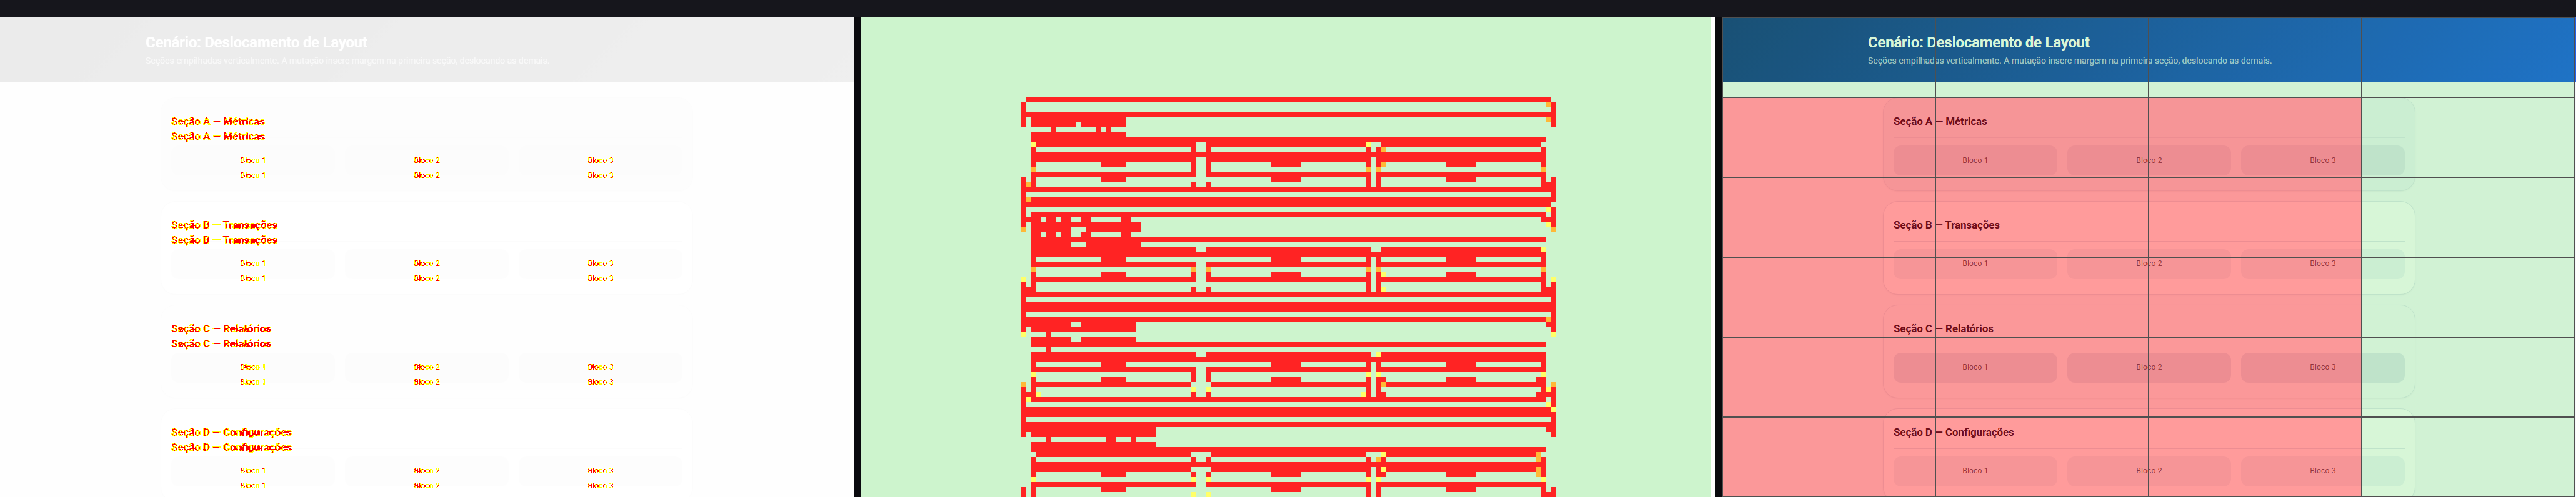
\includegraphics[width=\linewidth]{Figs/06-painel-layout.png}
\label{fig:painel-layout}
\end{center}
\flushleft
\vspace{-0.5cm}
\hspace{0.08cm} \footnotesize{ Fonte: Do autor.}
\end{figure}

A Figura~\ref{fig:painel-opacidade} ilustra o caso oposto: uma alteração real que não aciona nenhuma das três técnicas. A redução de opacidade para 0,92 em três dos seis cards alterou cada pixel individualmente em magnitude inferior à tolerância por canal de pixelmatch (0,1), de modo que nenhum pixel foi contado como divergente; a SSIM ficou em 0,9996 (estrutura preservada) e nenhuma célula ultrapassou 1\,\%. O resultado exemplifica o equilíbrio entre sensibilidade e ruído: limiares mais permissivos reduzem alertas indevidos, mas podem deixar passar variações visíveis de baixa amplitude.

\begin{figure}[H]
\begin{center}
\captionlistentry{}
Figura \thefigure \hspace{1pt} - Cenário \emph{Opacidade}: alteração existe, mas permanece abaixo dos limiares nas três técnicas
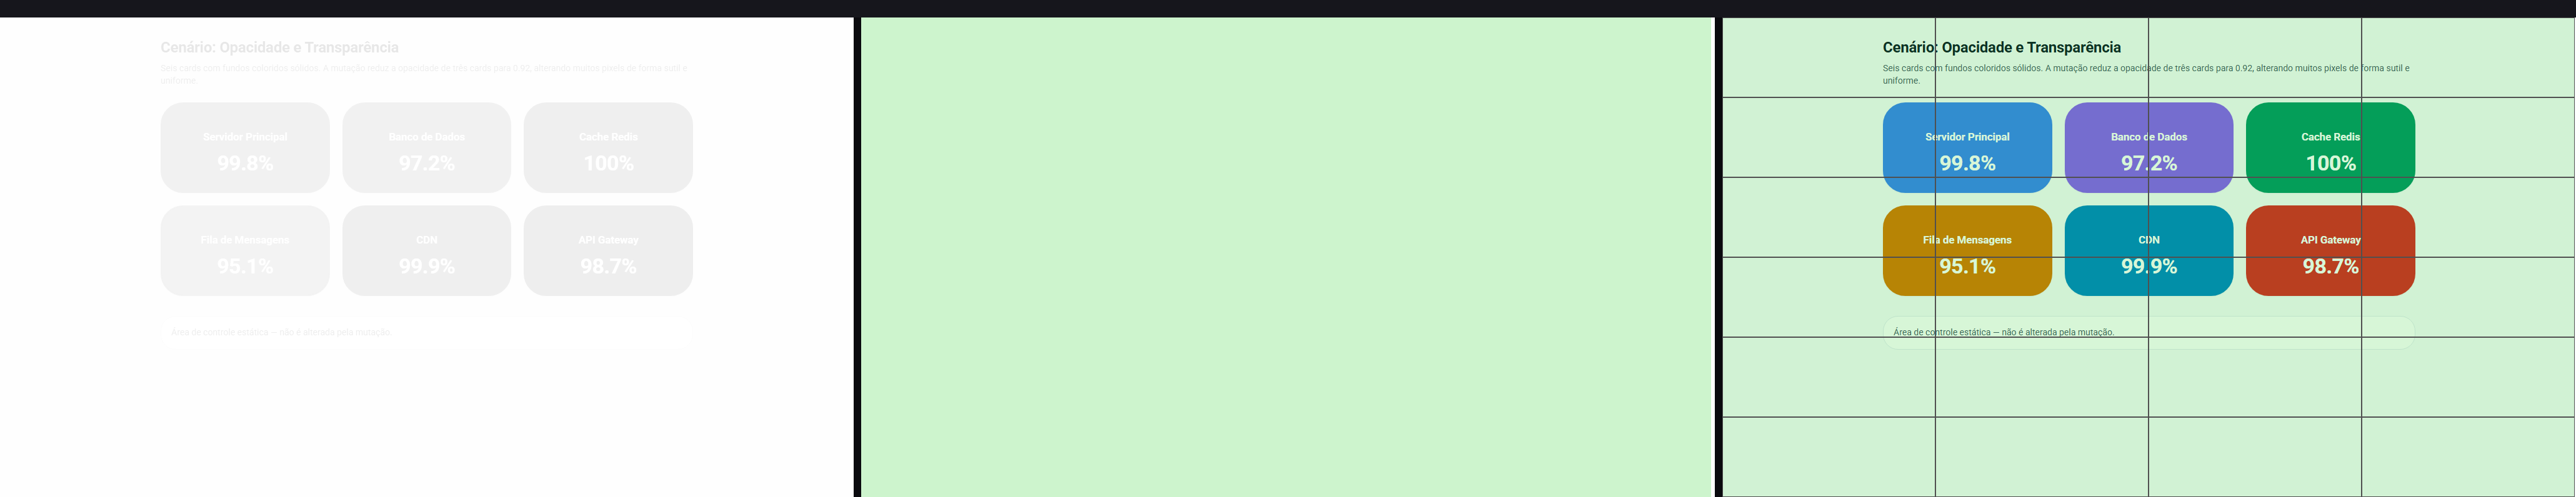
\includegraphics[width=\linewidth]{Figs/07-painel-opacidade.png}
\label{fig:painel-opacidade}
\end{center}
\flushleft
\vspace{-0.5cm}
\hspace{0.08cm} \footnotesize{ Fonte: Do autor.}
\end{figure}

A Figura~\ref{fig:painel-microshift} expõe o limite inferior de detecção. Um deslocamento de apenas 1\,px gerou 0,198\,\% de pixels diferentes, queda da SSIM para 0,9316 e 14 células reprovadas em 24. A queda da SSIM é mais expressiva do que a magnitude sugere porque, ao deslocar verticalmente uma sequência de blocos, cada janela da grade passa a comparar pixels desalinhados, afetando luminância e contraste localmente. No experimento, pequenas translações produziram assinaturas amplas nas três técnicas; SSIM e regiões ofereceram leitura mais informativa sobre a natureza estrutural do efeito do que a simples contagem de pixels divergentes.

\begin{figure}[H]
\begin{center}
\captionlistentry{}
Figura \thefigure \hspace{1pt} - Cenário \emph{Micro-deslocamento (1\,px)}: as três técnicas reprovam, com perfis diferentes
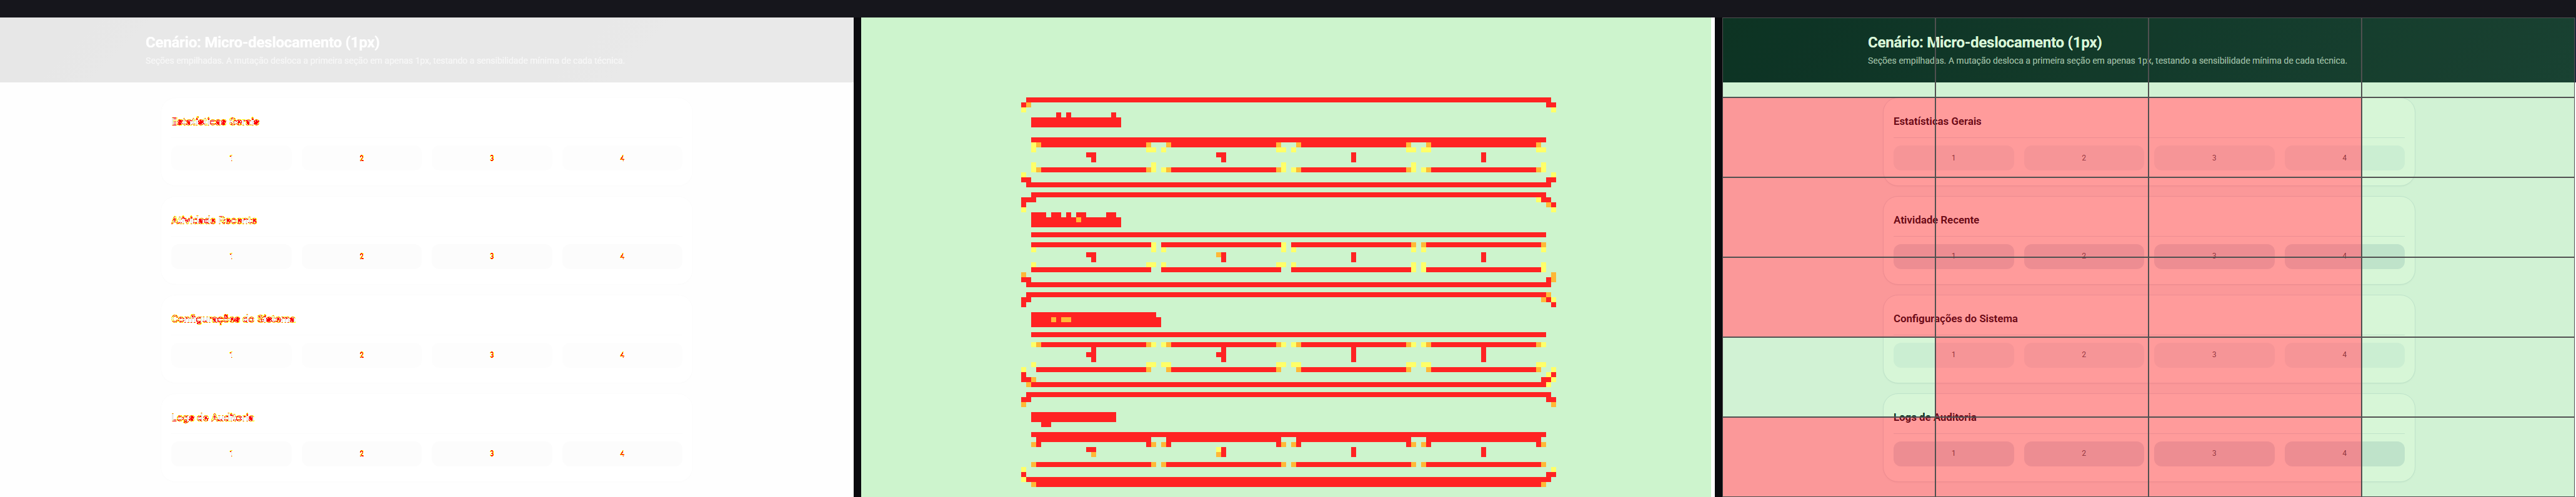
\includegraphics[width=\linewidth]{Figs/08-painel-microshift.png}
\label{fig:painel-microshift}
\end{center}
\flushleft
\vspace{-0.5cm}
\hspace{0.08cm} \footnotesize{ Fonte: Do autor.}
\end{figure}

A Figura~\ref{fig:painel-dinamico} ilustra a situação em que a tela contém um valor que muda a cada execução (data, contador) sem que isso represente uma regressão. As técnicas pixel e SSIM aprovaram a captura, com 0,064\,\% de pixels diferentes e 0,9979 de pontuação, porque a variação ocupa uma fração muito pequena da imagem total. A abordagem por regiões reprovou a célula que contém o valor variável, porque dentro daquele quadrante isolado a porcentagem de pixels modificados ultrapassou o limiar local de 1\,\%. O resultado mostra a vantagem de avaliar a imagem por partes em vez da média da imagem inteira, já que defeitos pequenos não ficam diluídos. Justifica também a aplicação de máscara na célula correspondente em vez de aumentar globalmente o limiar do pixel, pois a estratégia preserva a capacidade de detecção no restante da tela e neutraliza apenas o ponto sabidamente variável.

\begin{figure}[H]
\begin{center}
\captionlistentry{}
Figura \thefigure \hspace{1pt} - Cenário \emph{Conteúdo dinâmico} sem máscara: apenas a técnica por regiões isola a célula variável
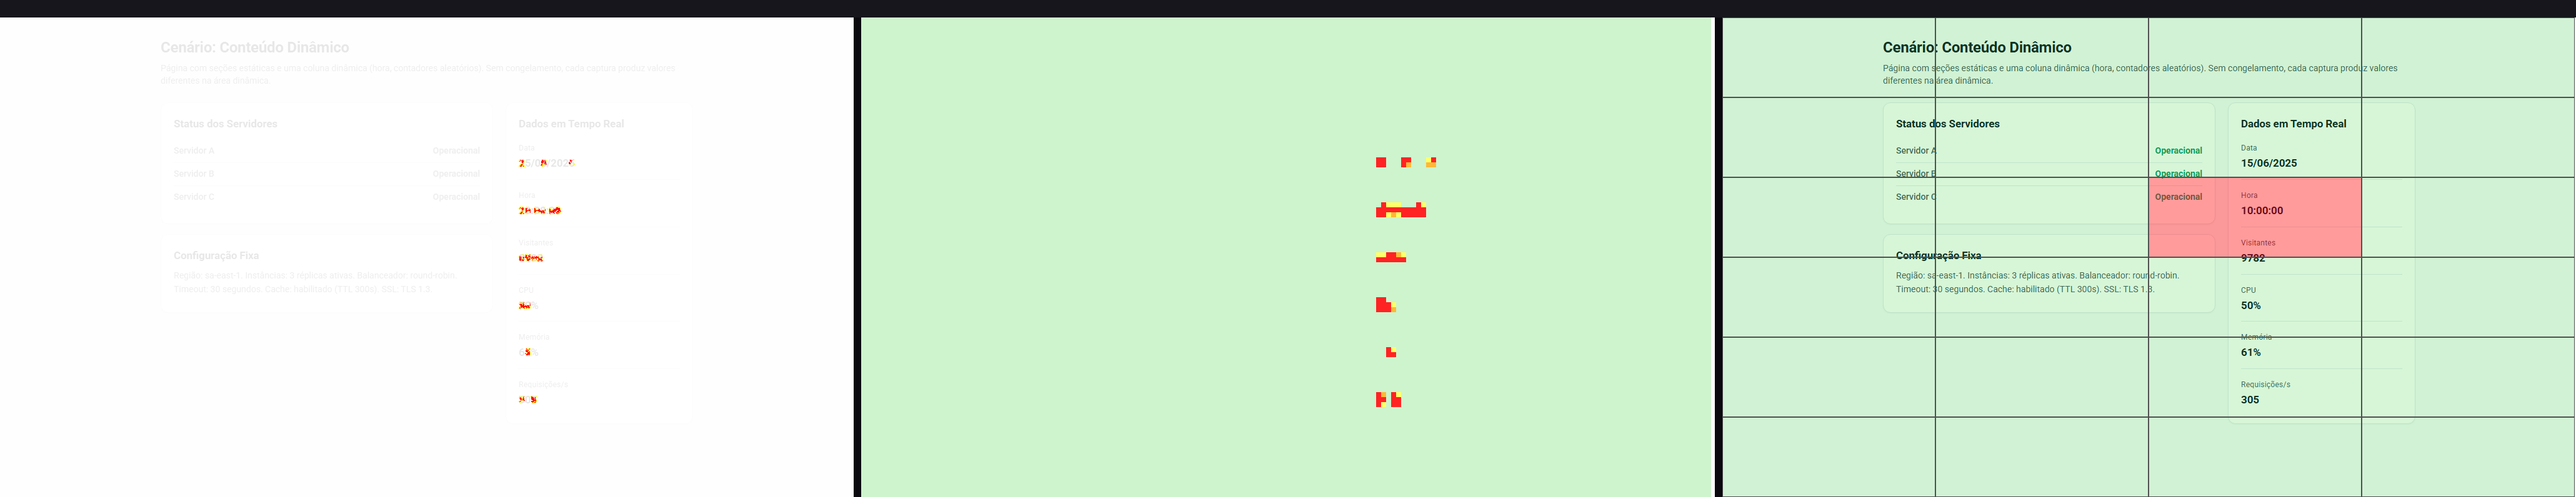
\includegraphics[width=\linewidth]{Figs/09-painel-dinamico.png}
\label{fig:painel-dinamico}
\end{center}
\flushleft
\vspace{-0.5cm}
\hspace{0.08cm} \footnotesize{ Fonte: Do autor.}
\end{figure}



\subsection{COMPARAÇÃO POR CENÁRIOS DE REGRESSÃO}
A Tabela~\ref{tab:cenarios} apresenta os resultados da avaliação por cenários. Cada linha corresponde a um tipo de mutação controlada, e as colunas indicam o veredito e a métrica principal de cada técnica.

\vspace{0.2cm}
\begin{table}[H]
\centering
\captionlistentry{}
Tabela \thetable  \hspace{0.5pt} - {Resultados por cenário de regressão (\emph{viewport} 1366\,$\times$\,768\,px)}
\label{tab:cenarios}
\resizebox{\textwidth}{!}{%
\begin{tabular}{p{6cm}|c|c|c}
\hline
\multicolumn{4}{c}{\textbf{Resultados por cenário de regressão (viewport 1366$\times$768\,px)}} \\
\hline
\textbf{Cenário} & \textbf{Pixel (\%diff)} & \textbf{SSIM (score)} & \textbf{Regiões (falhas)} \\
\hline
Mudança sutil de cor       & FAIL (5,854\%) & PASS (0,9976) & FAIL (8/24) \\
\hline
Deslocamento de layout     & FAIL (0,637\%) & FAIL (0,8762) & FAIL (15/24) \\
\hline
Variação tipográfica       & FAIL (2,186\%) & FAIL (0,9269) & FAIL (13/24) \\
\hline
Conteúdo dinâm. (s/ másc.) & PASS (0,064\%) & PASS (0,9979) & FAIL (1/24) \\
\hline
Conteúdo dinâm. (c/ másc.) & PASS (0,064\%) & PASS (0,9979) & PASS (0/24) \\
\hline
Alteração de componente    & FAIL (0,128\%) & PASS (0,9924) & FAIL (1/24) \\
\hline
Opacidade e transparência  & PASS (0\%)     & PASS (0,9996) & PASS (0/24) \\
\hline
Sombra e elevação          & PASS (0\%)     & PASS (0,9953) & PASS (0/24) \\
\hline
Micro-deslocamento (1\,px) & FAIL (0,198\%) & FAIL (0,9316) & FAIL (14/24) \\
\hline
Alteração de borda fina    & FAIL (0,273\%) & PASS (0,9998) & FAIL (4/24) \\
\hline
Remoção de elemento        & FAIL (0,399\%) & FAIL (0,9822) & FAIL (3/24) \\
\hline
Troca de família de fonte  & FAIL (2,614\%) & FAIL (0,8886) & FAIL (14/24) \\
\hline
Imagem idêntica (controle) & PASS (0\%)     & PASS (1,0000) & PASS (0/24) \\
\hline
\end{tabular}%
}
\vspace{-0.3cm}
\flushleft
\hspace{0cm}\footnotesize Fonte: Do autor.
\end{table}

A leitura da Tabela~\ref{tab:cenarios} permite identificar três grupos distintos de comportamento, cada um associado a um tipo de alteração na interface.

O primeiro grupo é o das alterações que afetam a relação espacial ou estrutural dos elementos, em que as três técnicas reprovaram simultaneamente: deslocamento de \emph{layout}, variação tipográfica, troca de fonte, micro-deslocamento e remoção de elemento. A SSIM caiu para 0,8762 (deslocamento), 0,9269 (tipografia), 0,8886 (troca de fonte), 0,9316 (micro-deslocamento) e 0,9822 (remoção), enquanto a abordagem por regiões apontou 15, 13, 14, 14 e 3 células reprovadas em 24, respectivamente. No cenário de remoção, a queda da SSIM é menos intensa do que nos demais porque o efeito estrutural se concentra em uma fração da imagem, mas ainda supera o limiar de 0,99. Mudanças que alteram a estrutura perceptual da tela, seja por deslocamento, por recomposição tipográfica ou por supressão de conteúdo, são detectadas pelas três abordagens. O padrão coincide com a caracterização da SSIM em \citeonline{wang2004} e com a observação de \citeonline{tanno2020} de que essas mudanças se traduzem em diferenças amplas ou localmente intensas na imagem.

O segundo grupo é o das alterações localizadas de natureza predominantemente cromática, em que pixel e regiões reprovaram e a SSIM aprovou: troca de cor de borda fina e alteração de texto e cor de borda em um único componente. Os percentuais de pixel são pequenos (0,273\,\% e 0,128\,\%), mas ultrapassaram o limiar de 0,1\,\% e acionaram o alerta. A SSIM ficou acima de 0,99 e aprovou as duas (0,9998 e 0,9924), porque a variação é cromática e não altera contornos, formas ou contraste estrutural. A abordagem por regiões reprovou as duas (4/24 e 1/24), fornecendo informação espacial que reduz a inspeção a poucos quadrantes. Nesses casos, a SSIM isolada deixaria passar mudanças visíveis; a combinação entre pixel e regiões corrige essa limitação tanto detectando quanto localizando. Note-se que o cenário de mudança sutil de cor, discutido em seção anterior, apresenta comportamento análogo (SSIM 0,9976 $>$ 0,99, aprovado; pixel e regiões reprovados) e poderia compor este grupo, mas foi destacado nas evidências visuais por ilustrar com mais clareza a complementaridade das técnicas.

O terceiro grupo reúne cenários em que a alteração foi injetada, mas sua amplitude na imagem renderizada ficou abaixo dos limiares: opacidade 0,92 (pixel 0\,\%, SSIM 0,9996, 0/24) e \emph{box-shadow} em três cards (pixel 0\,\%, SSIM 0,9953, 0/24). O resultado decorre de duas limitações sobrepostas: a própria mutação produziu variação por canal inferior à tolerância de pixelmatch, e os limiares adotados não foram calibrados para variações de baixa amplitude. A SSIM 0,9953 da sombra indica queda estrutural detectável e seria reprovada com limiar 0,996, em linha com a discussão de \citeonline{tanno2020} sobre o equilíbrio entre sensibilidade e ruído.

A tabela responde à lacuna apontada na introdução. \citeonline{tanno2020} e \citeonline{heinonen2020} discutem técnicas e ambiente, mas não apresentam comparação numérica por cenário rotulado, e este trabalho apresenta esse recorte com valores extraídos automaticamente pelo fluxo PixelGuard. \citeonline{figueiredo2018} e \citeonline{bordignon2019} demonstraram, no contexto nacional, a viabilidade de testes visuais em projetos Android e na avaliação de ferramentas de interface, mas não conduziram cenários de mutação controlada com coleta de métricas por técnica nem integraram os resultados a um fluxo rastreável de CI/CD, lacuna que este trabalho preenche ao executar os três métodos em cenários rotulados com evidências vinculadas ao histórico de versões. O cenário de conteúdo dinâmico, executado nas duas variantes, complementa o recorte ao mostrar como a aplicação de máscara restrita altera o resultado. Sem máscara, a abordagem por regiões reprovou por ruído em uma única célula. Com máscara aplicada apenas à célula afetada, todas as 24 regiões foram aprovadas, sem esconder o restante da tela. O comportamento confirma que máscaras pontuais, revisadas a cada atualização de \emph{baseline}, neutralizam ruído de conteúdo variável sem comprometer a cobertura do restante da tela.

\subsection{SÍNTESE COMPARATIVA}
A avaliação por treze cenários (doze com mutação e um de controle) indicou que cada técnica apresenta um perfil distinto de detecção e que as abordagens são complementares entre si. A Tabela~\ref{tab:sintese} resume o comportamento por tipo de alteração.

\vspace{0.2cm}
\begin{table}[H]
\centering
\captionlistentry{}
Tabela \thetable  \hspace{0.5pt} - {Síntese de detecção por técnica e tipo de alteração}
\label{tab:sintese}
\resizebox{\textwidth}{!}{%
\begin{tabular}{p{6cm}|c|c|c}
\hline
\multicolumn{4}{c}{\textbf{Síntese de detecção por técnica e tipo de alteração}} \\
\hline
\textbf{Tipo de alteração} & \textbf{Pixel} & \textbf{SSIM} & \textbf{Regiões} \\
\hline
Cor sutil          & Detecta & Não detecta & Detecta \\
\hline
Deslocamento       & Detecta & Detecta     & Detecta \\
\hline
Tipografia         & Detecta & Detecta     & Detecta \\
\hline
Dinâmico (s/ másc.)& Não detecta & Não detecta & Detecta \\
\hline
Dinâmico (c/ másc.)& Não detecta & Não detecta & Não detecta \\
\hline
Componente local   & Detecta & Não detecta & Detecta \\
\hline
Opacidade          & Não detecta & Não detecta & Não detecta \\
\hline
Sombra             & Não detecta & Não detecta & Não detecta \\
\hline
Micro-deslocamento (1 px) & Detecta & Detecta     & Detecta \\
\hline
Borda fina         & Detecta & Não detecta & Detecta \\
\hline
Remoção de elemento& Detecta & Detecta     & Detecta \\
\hline
Troca de fonte     & Detecta & Detecta     & Detecta \\
\hline
Controle (idêntico)& Sem falso+ & Sem falso+ & Sem falso+ \\
\hline
\end{tabular}%
}
\vspace{-0.3cm}
\flushleft
\hspace{0cm}\footnotesize Fonte: Do autor.
\end{table}

A comparação \emph{pixel a pixel} detectou oito dos doze cenários com mutação. A SSIM detectou cinco. A abordagem por regiões detectou nove, com melhor apoio à localização da diferença. Em conjunto, os dados mostram que não há técnica única suficiente para todos os tipos de alteração. A taxa de detecção observada por técnica (8/12, 5/12 e 9/12) é coerente com o quadro descrito por \citeonline{tanno2020}, em que a comparação direta cobre bem mudanças visíveis e localizadas, a SSIM cobre principalmente mudanças que afetam estrutura, e a abordagem por regiões oferece o melhor compromisso entre detecção e suporte à triagem, especialmente quando há necessidade de mascarar áreas dinâmicas.

O fluxo que combina as três técnicas atendeu melhor aos objetivos da pesquisa. O pixel ofereceu sensibilidade, a SSIM ofereceu leitura perceptual da severidade e a abordagem por regiões ofereceu contexto espacial e controle de conteúdo dinâmico. A combinação reduziu o risco de decisão baseada em um único indicador. Frente aos correlatos, este trabalho avança em quatro pontos. O primeiro é a execução dos três métodos sob mesma calibração em treze cenários rotulados, suprindo a lacuna de comparação numérica apontada em \citeonline{tanno2020}. O segundo é a integração a um \emph{pipeline} real de CI/CD com artefatos rastreáveis (relatório HTML, \emph{Review UI} e \emph{Statuses} do GitHub), na linha do que \citeonline{heinonen2020} recomenda. O terceiro é a manutenção do determinismo do ambiente, conforme \citeonline{wang2004} e \citeonline{heinonen2020}, o que garante que os indicadores observados refletem a mutação injetada e não ruído de captura. O quarto é a extensão ao contexto de aplicações web com integração a CI/CD, alcançando um recorte não coberto por \citeonline{figueiredo2018}, que avaliou VRT em Android sem pipeline de CI, nem por \citeonline{bordignon2019}, que analisou ferramentas de teste de interface sem cenários de mutação com coleta de métricas por técnica.

\section{CONCLUSÃO}

Este trabalho avaliou três técnicas de regressão visual, comparação \emph{pixel a pixel}, SSIM e abordagem por regiões, dentro de um fluxo automatizado de CI/CD com geração de evidências rastreáveis. Com a implementação da PixelGuard e a execução de treze cenários controlados, foi possível comparar capacidade de detecção, ruído e apoio à triagem.

Os resultados mostram que nenhuma técnica, isoladamente, cobre todos os tipos de mudança avaliados. A comparação \emph{pixel a pixel} foi mais sensível a diferenças pontuais (oito cenários detectados). A SSIM identificou cinco cenários, cobrindo principalmente mudanças estruturais e de remoção. A abordagem por regiões obteve o maior índice de detecção (nove cenários), com melhor apoio à triagem por indicar em que região da tela a diferença ocorreu e por permitir mascaramento de conteúdo dinâmico.

No cenário de controle, as três técnicas aprovaram corretamente, sem falso positivo. Nos cenários com mutação, a detecção variou conforme o tipo de alteração. Mudanças estruturais foram detectadas com mais consistência. Alterações de baixo contraste, como redução de opacidade para 0,92 e adição de sombra leve, não foram detectadas em nenhuma das três técnicas. O resultado expressa duas limitações sobrepostas, a magnitude reduzida da própria mutação (que ficou abaixo da tolerância por canal da comparação \emph{pixel a pixel}) e a permissividade dos limiares adotados, e indica tanto a necessidade de calibração dos parâmetros de aceitação quanto a conveniência de mutações de maior amplitude em ampliações futuras do conjunto de cenários.

Confirmou-se, adicionalmente, a importância do determinismo no ambiente de captura. O congelamento do relógio e da função Math.random, em conjunto com o controle de animações, idioma, fuso horário e dimensão do \emph{viewport}, reduziu instabilidades entre execuções e garantiu que os indicadores mensurados refletem a mutação injetada, e não ruído de captura, condição necessária para que as métricas sejam interpretadas com validade interna.

A combinação das três técnicas no mesmo \emph{pipeline} foi a estratégia que apresentou melhor equilíbrio entre sensibilidade, interpretação dos resultados e suporte à decisão em solicitações de mudança. As principais limitações do estudo são o escopo em uma única aplicação de página única (\emph{single-page}), o que restringe a generalização para outros contextos, a execução dos doze cenários de mutação em apenas um \emph{viewport} (1366\,$\times$\,768\,px), enquanto a avaliação multi-\emph{viewport} ficou restrita à tela \textit{dashboard}, e a ausência de cronometragem do esforço de triagem com avaliadores, já que esse aspecto foi observado de forma qualitativa pelas evidências geradas no fluxo.

A principal lição aprendida no desenvolvimento do trabalho é que o determinismo do ambiente de captura não é detalhe de implementação, mas pré-condição para a validade dos resultados: qualquer fonte de variação não controlada entre capturas invalida a comparação independentemente da técnica utilizada. A segunda lição é que limiares configuráveis são mais úteis do que limiares fixos otimizados para um único conjunto de dados, pois o perfil de ruído varia por aplicação, resolução e tecnologia de renderização.

Os objetivos específicos foram atendidos. Identificaram-se doze tipos de mutação controlada, abrangendo variações cromáticas, estruturais, tipográficas e de conteúdo dinâmico; o fluxo automatizado foi implementado no GitHub Actions com relatório HTML, interface de revisão e integração com a API de \emph{Statuses}; e o desempenho das técnicas foi mensurado por indicadores extraídos automaticamente (pixel: 8/12 cenários detectados; SSIM: 5/12; regiões: 9/12; zero falso positivo no controle).

Como trabalhos futuros, recomenda-se ampliar a avaliação para outras aplicações além de uma única \emph{single-page}, em domínios distintos. Outra direção é estender a comparação a cenários de acessibilidade (simulação de daltonismo, baixa visão e alto contraste) e à paridade entre navegadores e dispositivos para a mesma versão da página. Recomenda-se também conduzir a varredura sistemática dos limiares por meio de curva ROC sobre conjunto rotulado, para subsidiar uma escolha quantitativamente fundamentada dos parâmetros de aceitação de cada técnica.

\bibliographystyle{abntex2-unesc}
\renewcommand{\refname}{REFERÊNCIAS}
\bibliography{referencias}

\end{document}
